
\documentclass[10pt,a4paper,twocolumn,twoside]{article}
\usepackage[utf8]{inputenc}
\usepackage[catalan]{babel}
\usepackage{multicol}
\usepackage{graphicx}
\usepackage{fancyhdr}
\usepackage{times}
\usepackage{titlesec}
\usepackage{multirow}
\usepackage{lettrine}
\usepackage[top=2cm, bottom=1.5cm, left=2cm, right=2cm]{geometry}
\usepackage[figurename=Fig.,tablename=TAULA]{caption}
\usepackage{svg}
\captionsetup[table]{textfont=sc}

\author{\LARGE\sffamily Pau Casacuberta Orta}
\title{\Huge{\sffamily Disseny d'un ``core'' RISC-V Didàctc}}
\date{}

\newcommand\blfootnote[1]{%
  \begingroup
  \renewcommand\thefootnote{}\footnote{#1}%
  \addtocounter{footnote}{-1}%
  \endgroup
}

%
%\large\bfseries\sffamily
\titleformat{\section}
{\large\sffamily\scshape\bfseries}
{\textbf{\thesection}}{1em}{}

\begin{document}

\fancyhead[LO]{\scriptsize Pau Casacuberta Orta: Disseny d'un ``core'' RISC-V Didàctc}
\fancyhead[RO]{\thepage}
\fancyhead[LE]{\thepage}
\fancyhead[RE]{\scriptsize EE/UAB TFG INFORMÀTICA: Disseny d'un ``core'' RISC-V Didàctc}

\fancyfoot[CO,CE]{}

\fancypagestyle{primerapagina}
{
   \fancyhf{}
   \fancyhead[L]{\scriptsize TFG EN ENGINYERIA INFORMÀTICA, ESCOLA D'ENGINYERIA (EE), UNIVERSITAT AUTÒNOMA DE BARCELONA (UAB)}
   \fancyfoot[C]{\scriptsize Febrer de 2020, Escola d'Enginyeria (UAB)}
}

%\lhead{\thepage}
%\chead{}
%\rhead{\tiny EE/UAB TFG INFORMÀTICA: TÍTOL (ABREUJAT SI ÉS MOLT LLARG)}
%\lhead{ EE/UAB \thepage}
%\lfoot{}
%\cfoot{\tiny{February 2015, Escola d'Enginyeria (UAB)}}
%\rfoot{}
\renewcommand{\headrulewidth}{0pt}
\renewcommand{\footrulewidth}{0pt}
\pagestyle{fancy}

%\thispagestyle{myheadings}
\twocolumn[\begin{@twocolumnfalse}

%\vspace*{-1cm}{\scriptsize TFG EN ENGINYERIA INFORMÀTICA, ESCOLA D'ENGINYERIA (EE), UNIVERSITAT AUTÒNOMA DE BARCELONA (UAB)}

\maketitle

\thispagestyle{primerapagina}
%\twocolumn[\begin{@twocolumnfalse}
%\maketitle
%\begin{abstract}
\begin{center}
\parbox{0.915\textwidth}
{\sffamily
\textbf{Resum--}
Resum del projecte, màxim 10 línies. ........ ........... .......... ..  ... ..... .... ........ ........... .......... ..  ... ..... .... ........ ........... .......... ..  ... ..... .... ........ ........... .......... ..  ... ..... .... ........ ........... .......... ..  ... ..... .... ........ ........... .......... ..  ... ..... .... ........ ........... .......... ..  ... ..... .... ........ ........... .......... ..  ... ..... .... ........ ........... .......... ..  ... ..... .... ........ ........... .......... ..  ... ..... .... ........ ........... .......... ..  ... ..... .... .................. ..  ... ..... .... ........ ........... .......... ..  ... ..... .... ........ ........... .......... ..  ... ..... .... ........ ........... .......... ..  ... ..... .... ........ ........... .......... ..  ... ..... .... ........ ........... .......... ..  ... ..... .... ........ ........ .......... ..  ... . ........... .......... ..  ... ..... .... ........ ........... .......... ..  ... ..... .... ........ ........... .......... ..  ... ..... .... ........ ........... .......... ..  ... ........... ..  ... ..... .... ........ ........... .......... ..  ... ..... .... ........ ........... .......... ..  ... ..... .... ........ ........... .......... ..  ... ..... .... ........ ........... .......... ..  ... ..... .... ........ ........... .......... ..  ... ..... .... ........ ........... .......... ..  ... ..... .... ........ ........... .......... ..  ... ..... .... ........ ........... .......... ..  ... ..... .... 
\\
\\
\textbf{Paraules clau-- } Paraules clau del treball, màxim 2 línies . .... ........ ........... .......... ..  ... ..... .... ........ ........... .......... ..  ... ..... .... ........ ........... ................\\
\\
%\end{abstract}
%\bigskip
%\begin{abstract}
\bigskip
\\
\textbf{Abstract--} Versió en anglès del resum . ........ ........... .......... ..  ... ..... .... ........ ........... .......... ..  ... ..... .... ........ ........... .......... ..  ... ..... .... ........ ........... .......... ..  ... ..... .... ........ ........... .......... ..  ... ..... .... ........ ........... .......... ..  ... ..... .... ........ ........... .......... ..  ... ..... .... ........ ........... .......... ..  ... ..... .... ........ ........... .......... ..  ... ..... .... ........ ........... .......... ..  ... ..... .... ........ ........... .......... ..  ... ..... .... .................. ..  ... ..... .... ........ ........... .......... ..  ... ..... .... ........ ........... .......... ..  ... ..... .... ........ ........... .......... ..  ... ..... .... ........ ........... .......... ..  ... ..... .... ........ ........... .......... ..  ... ..... .... ........ ........ .......... ..  ... . ........... .......... ..  ... ..... .... ........ ........... .......... ..  ... ..... .... ........ ........... .......... ..  ... ..... .... ........ ........... .......... ..  ... ........... ..  ... ..... .... ........ ........... .......... ..  ... ..... .... ........ ........... .......... ..  ... ..... .... ........ ........... .......... ..  ... ..... .... ........ ........... .......... ..  ... ..... .... ........ ........... .......... ..  ... ..... .... ........ ........... .......... ..  ... ..... .... ........ ........... .......... ..  ... ..... .... ........ ........... .......... ..  ... ..... .... 
\\
\\
\textbf{Keywords-- } Versió en anglès de les paraules clau. .... ........ ........... .......... ..  ... ..... .... ........ ........... .......... ..  ... ..... .... ........ ........... .................. ..\\
}

\bigskip

{\vrule depth 0pt height 0.5pt width 4cm\hspace{7.5pt}%
\raisebox{-3.5pt}{\fontfamily{pzd}\fontencoding{U}\fontseries{m}\fontshape{n}\fontsize{11}{12}\selectfont\char70}%
\hspace{7.5pt}\vrule depth 0pt height 0.5pt width 4cm\relax}

\end{center}

\bigskip
%\end{abstract}
\end{@twocolumnfalse}]

\blfootnote{$\bullet$ E-mail de contacte: pau.casacubertao@e-campus.uab.cat}
\blfootnote{$\bullet$ Menció realitzada: Enginyeria de Computadors }
\blfootnote{$\bullet$ Treball tutoritzat per: nom i cognoms del tutor (departament)}
\blfootnote{$\bullet$ Curs 2019/20}

\section{Introducció}
%Secció d’introducció on es motiva el treball i es plantegen els objectius, i també s’explica breument l’organització de la resta del document.
\lettrine[lines=3]{E}{n} el disseny d'arquitectures de computadors la part més important a l'hora de construir aquest és l'elecció d'un conjunt d'instruccions que aquest podrà executar, ja que a partir de les operacions bàsiques es farà el disseny del propi nucli i dels mòduls que el conformen. 
El repertori es la manera de poder generar programes que després podrà executar el processador.  trobem dos jocs d'instruccions principals a l'hora de dissenyar processadors per a ordinadors. 
Els principals jocs d'instruccions per a processadors d'us generals (ordinadors personals i dispositius mòbils) són x86 i ARM, on cada una té dissenys diferents i si es vol utilitzar per a algun futur dispositius s'ha de llicenciar l'us.

Ara bé, per canviar aquest entorn limitat d'opcions propietàries fa uns anys ha anat creixent una iniciativa, iniciada a la Universitat de Califòrnia a Berkeley \cite{krste_asanovic_instruction_2014}, que proposa un disseny de processador obert i lliure, això ho aconsegueix alliberant el repertori d'instruccions, en anglès ISA (Instruction Set Architecture), al public. Això permet que qualsevol universitat o empresa pugui crear una arquitectura a partir d'aquest repertori lliure de royalties i amb l'opció de poder-se involucrar en el desenvolupament, iniciant un camí cap al hardware obert i lliure. 

Aquesta nova arquitectura es diu RISCV i últimament està dominant les tendències i estratègies de futur i prometen una ràpida expansió.

Aquest Treball Fi de Grau pretén proposar un disseny d'un nucli de processador RISCV amb l’objectiu d’anar avançant cap un entorn didàctic per a conèixer aquest tipus de processador, des del propi nucli del processador fins a un entorn gràfic que permeti mostrar l'execució de programes escrits en C, indicant quines parts del nucli es fan servir.
Tot això com a eina didàctica per a entendre el funcionament dels computadors amb conjunts d'instruccions actuals. 

Concretament la micro-arquitectura que s'implementarà consistirà en un subconjunt del repertori d’instruccions, el \textbf{ISA-RV32I}. 
Aquest nucli serà mono-cicle i d’execució seqüencial d’instruccions. 

A la secció \ref{sec:Obj} es detallen els objectius





\section{Objectius} 
\label{sec:Obj}
El principal objectiu d'aquest treball és produir un disseny d'un nucli RISCV a nivell RTL en Verilog on el codi sigui fàcil de seguir i provar que es funcional implementant-lo en una FPGA i executar programes compilats amb eines preparades per al repertori de RISCV.

Aquest objectiu el podem dividir en diferents sub-objectius:

\begin{itemize}

    \item Aprendre a dissenyar un computador des de zero fent recerca d'informació. Aquesta recerca es basarà en consultar els documents oficials sobre l'ISA de RISCV \cite{waterman_volume_2019} \cite{waterman_volume_2019-1}  així com altres llibres que es centren més en el disseny de nuclis de processadors \cite{patterson_computer_2018} o en el llenguatge de descripció de hardware utilitzat, en aquest cas Verilog \cite{li_implementing_2018}.
    
    \item Fer un disseny funcional de parts del nucli per verificar el funcionament amb Verilog.

    \item Especificar i dissenyar a nivell HDL-RTL un nucli RISC-V amb el subconjunt bàsic de l’ISA, el RV32I.
    
    \item Preparar un Testbench per a comprovar el funcionament del nucli.
    
    \item Proporcionar un Core de Risc-V funcional (que permeti l'execució de programes simples escrits en C) però fàcil d'entendre'n la descripció en HDL.
    
    \item Per aplicar altres coneixements de la carrera, utilitzar eines d'Integració Continua per a automatitzar gran part de la part de tests i preparar eines per a desenvolupar el codi del processador.
    
    \item Materialitzar i testejar el nucli anterior en una placa de desenvolupament basada en FPGA.
    
        
\end{itemize}

\section{Estat del Art}
        Mostrar Cores, i aplicacions 
        
        Diversos projectes de nuclis de RISCV, molts utilitzen altres llenguatges per a obtenir l'arxiu final en verilog i poden ser més difícils de seguir que un llenguatge d'HDL.
        
        Plataformes que permeten entorn per a nuclis RISCV.
%\section{Finalitat del projecte}

\section{Core Risc-V}
A l'hora de dissenyar la micro-arquitectura del processador és important analitzar bé el repertori d'instruccions per a definir els elements que seran necessaris per a poder executar cada una d'aquestes instruccions.

A part del repertori d'instruccions qualsevol processador ha de tenir la possibilitat de poder emmagatzemar dades en \textbf{registres interns} i poder identificar cada línia de programa amb un altre registre anomenat\textbf{ Program Counter}.
En aquesta secció es descriurà en detall cada part del nucli. 
    \subsection{Instruction set}
    Per a dissenyar un nucli de processador primer s'ha de determinar quin repertori d'instruccions haurà d'executar, per aquest motiu a continuació es descriu com està composat el repertori RV32I utilitzat per al disseny del nucli en qüestió.
        %\subsubsection{RV32I}
    S'ha escollit el repertori RV32I degut a que és el més simple i permet fer operacions aritmeticològiques amb nombres enters, carregar i guardar dades a memòria externa, així com salts condicionals i incondicionals dins un programa.  
        
    Per a poder analitzar el conjunt d'instruccions aquestes es poden separar segons el tipus d'instrucció.
    
    \begin{figure}[!h]
    \centering
    	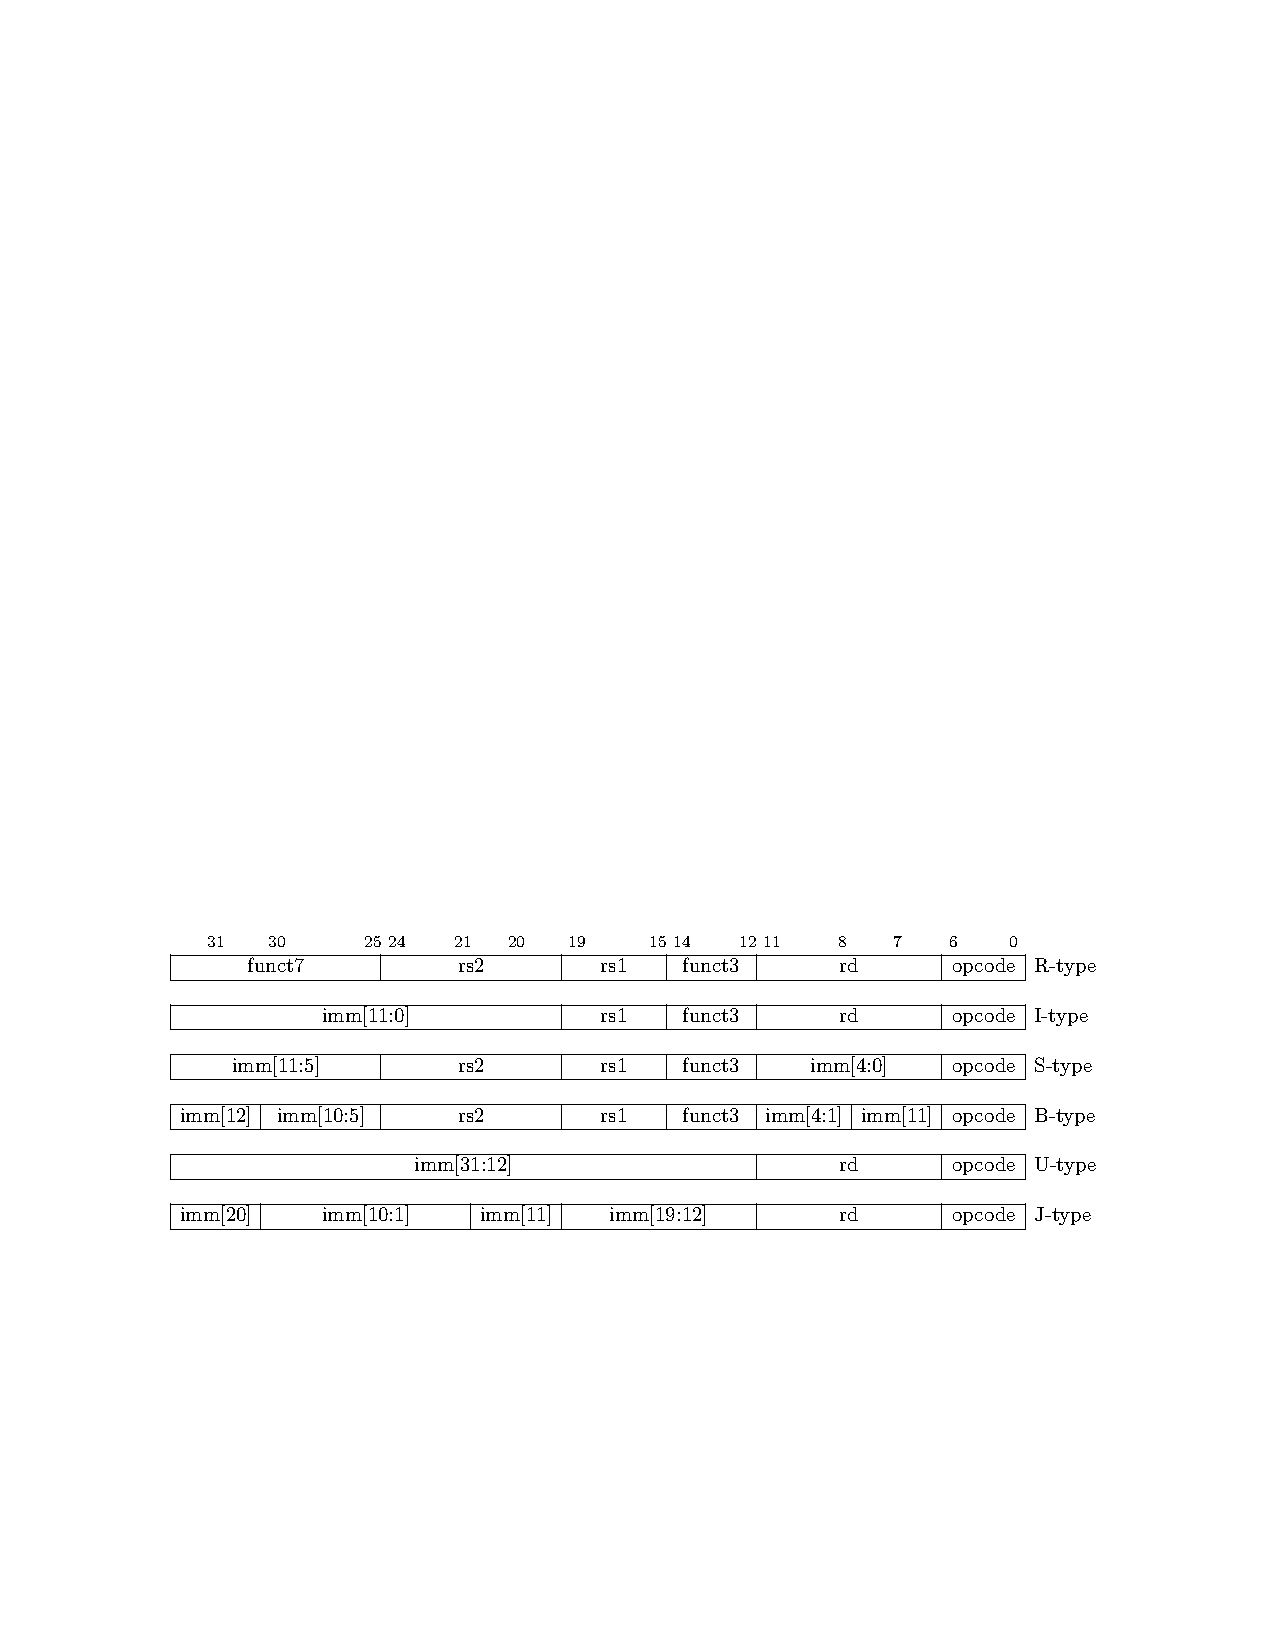
\includegraphics[width=\linewidth]{pdf/Encoding.pdf}
        \caption{RISC-V base instruction formats showing immediate variants.}
        \label{fig:baseinstformatsimm}
    \end{figure}
    
    En aquest proces de disseny s'ha decidit dividir les instruccions en quatre grups segons l'acció que s'efectua:
    
    \begin{itemize}
        \item Aritmeticològiques. Operacions que utilitzen valors instantanis o guardats en registres per a aplicar una operació aritmeticològica i guardar el resultat en un registre del banc de registres.
        \item Lectura o escriptura de dades a memòria externa. Operacions que a partir d'una adreça de memòria es guarda una dada de la memòria externa a un registre del banc de registres, o anàlogament guardar una dada d'un registre intern a una posició de memòria externa.
        \item Salts d'execució. Operacions que permeten modificar el valor del registre Comptador de Programa ja sigui després d'avaluar una comparació entre dos registres o de manera incondicional.
        \item Control del processador. Operacions relacionades amb registres d'estat i de control del processador i sistema d'interrupcions, en aquesta implementació no hi ha cap interrupció i els registres de control implementats son els mínims per complir amb l'especificació de RV32I en mode usuari.
    \end{itemize}
        
        
    
    \subsection{Arquitectura}
    \label{sec:arch}
    \begin{figure*}[!ht]
    \centering
    	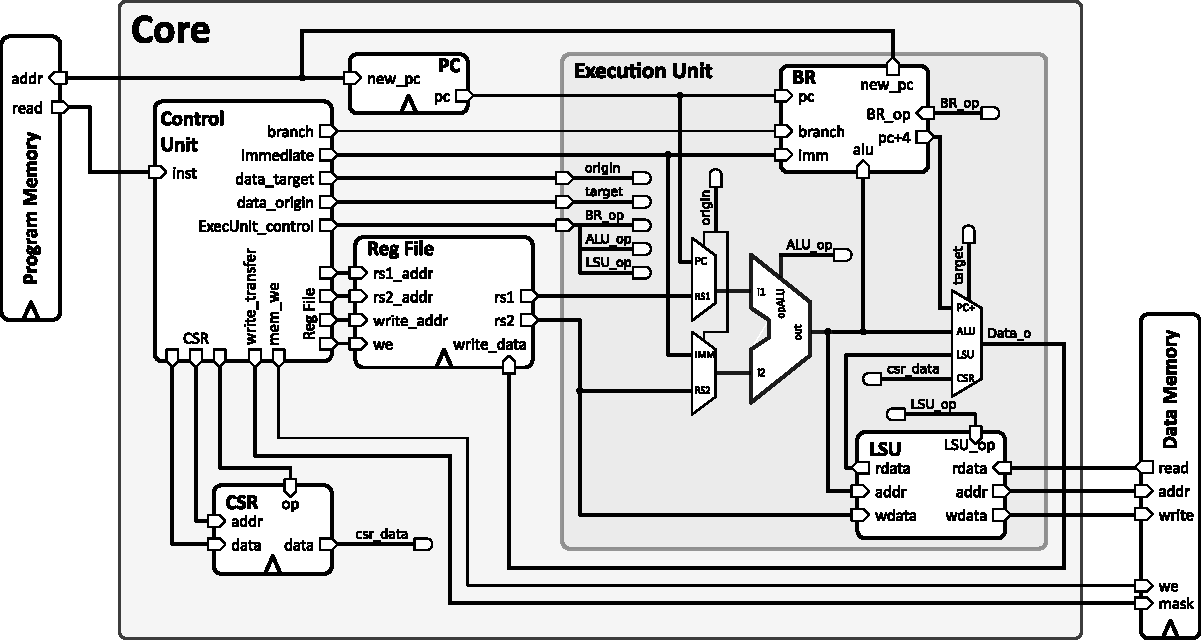
\includegraphics[width=0.9\linewidth]{pdf/arch_RiscV.pdf}
        \caption{Arquitectura del Nucli. Esquema de blocs de la distribució i connexions entre les diferents unitats i elements.}
        \label{fig:core_arch}
    \end{figure*}
    
    A la figura \ref{fig:core_arch} es pot veure un esquema de blocs general que mostra les unitats principals. Aquestes es poden diferenciar en dos tipus: les que implementen únicament lògica combinacional i les que també implementen lògica seqüencial (aquests tenen elements de memòria i necessiten d'un senyal de rellotge i de reinici).
    
    En el primer grup s'inclou la unitat de control, la unitat d'execució i dins d'aquesta les unitats de salt de programa, càrrega i escriptura de dades a memòria. Aquestes unitats es limiten a fer operacions de transformació de instruccions a senyals de control i dades (unitat de control), operacions aritmeticològiques (ALU), de càlcul de la següent adreça de programa (BR) o d'emmascarament de dades a l'hora d'accedir a memòria (LSU).
    
    En el segon grup s'inclou el comptador de programa, banc de registres, Unitat d'execució i la unitat de CSR.
    Aquestes unitats guarden dades d'
    i les mantenen fins al següent cicle de rellotge. 
    
    
    A les següents seccions es descriuen en detall les parts de l'arquitectura.
    \subsection{Senyals de Control}
    En aquesta secció es descriu quins senyals fan falta per a operar el core i els busos i línies de connexió interns que intercomuniquen les diferents unitats.
        
        %\subsubsection{Connexions externes}
        Els senyals bàsics per a poder operar el nucli des de l'exterior són:
        \begin{itemize}
            \item Els senyals de rellotge i reset: bàsics per a poder determinar la velocitat amb la que funcionarà aquest, és a dir cada quan els circuits seqüencials actualitzen les dades.
            \item Senyals relacionats amb les paraules de programa: conformats per un bus d'adreça (de com a molt 32 bits) que determina la posició en bytes de la següent línia de programa carregar i un altre bus (de 32 bits) que proporcionarà els 4 bytes que conformen una paraula de programa.
            \item Senyals relacionats amb la memòria de dades: conformats per un bus d'adreça (de com a molt 32 bits) que determina la posició en bytes de la dada que volem carregar o escriure, així com un bus de 4 bits que determina una màscara de quins bytes interessa modificar (per poder guardar un sol byte, mitja paraula o 2 bytes o una paraula sencera 4 bytes), també un senyal d'un bit per determinar si es vol escriure o llegir de la memòria i un altre bus (de 32 bits) que proporcionarà les dades que s'hagin d'escriure o llegir.
        \end{itemize}
        
        %\subsubsection{Senyals interns}
        Dins el Nucli a part de la distribució dels senyals de reinici i de rellotge a les unitats seqüencials trobem dos principals grups de senyals: els referent a les dades que s'estan utilitzant i els referents al control de les operacions que fa cada unitat.
        
        Els primers determinen valors immediats que s'obtenen directament de la instrucció base i descodificats segons el tipus tal i com es descriu a la figura \ref{fig:baseinstformatsimm}, en aquest grup podem incloure el valor "immediate" que surt directament de la unitat de control o el valor de csr\_data que surt de la mateixa unitat de control i arriba a la unitat de CSR, també serien els senyals rs1 i rs2 sortints del banc de registres o els senyals rdata i wdata de la unitat LSU. Dins aquest grup es podria afegir també el senyal de PC degut a que pot ser utilitzat com a senyal d'entrada per a operacions. La propietat en comú que tenen tots aquests senyals es que son de 32 bits i defineixen l'amplada de la paraula.
        
        En canvi per als senyals de control podem trobar diferents amplades de bus, per exemple els senyals referents a les adreces de l'accès a dades de memòria, així com els valors de rs1 i rs2 o de write\_addr per a determinar quins registres ha d'utilitzar el banc de registres així com el bus que determina l'adreça del registre CSR al qual es vol accedir. Per últim tenim la resta de senyals de control que determinen quin es el comportament de cada unitat, aquestes totes surten de la unitat de control i actuen sobre multiplexors com els senyals d'origin i target o busos que determinen quines operacions han d'executar cada un de les unitats com els senyals \verb|ALU_op|, \verb|BR_op|, \verb|LSU_op| o \verb|CSR_op|. En aquest últim grup podem incloure també els senyals de \verb|write_enable| que van tant al register file com a la memoria de dades.
        
        
        
        

        
        
        
        
        %*Senyals que determinen les operacions que han de fer altres mòduls (ALU, BR, LIS), senyals que informen de salts en el programa per a que diferents mòduls actuïn en consonància, senyals que indiquen adreces per llegir o escriure al banc de registres, senyals de control d'escriptura o lectura de dades al banc de registres, senyals que informen del comptador de programa de la instrucció actual.
        
    \subsection{Comptador de programa}
    
    El comptador de programa té la funció de mantenir el valor de l'adreça corresponent a la instrucció que s'està executant en un cicle de rellotge i poder utilitzar aquest valor per a determinar quina adreça següent demanar a la memòria de programa per a poder continuar l'execució.
    Degut a que aquest mòdul necessita guardar un valor és de tipus seqüencial necessita d'un senyal de rellotge per a determinar quan ha de carregar noves dades i de reinici  per a modificar el seu estat a un de conegut, habitualment 0 per a començar la execució d'un programa en aquesta adreça. 
    
    Aquest consisteix bàsicament d'un registre que emmagatzema el valor de la següent adreça de programa, normalment generada per la unitat de Branching, a cada cicle de rellotge i mantenir el valor durant aquest període per a que altres unitats l'utilitzin per definir la següent adreça a demanar o guardar-ne el valor en un registre.
    
    La implementació d'aquest mòdul en Verilog és molt senzilla ja que consisteix en assignar una dada d'entrada a un senyal de sortida registrat a cada cicle de rellotge o modificar el valor de dita sortia per 0 en el cas de detectar un senyal de reinici. 
    
    
    \subsection{Unitat de Control}
    *Mostrar esquema de la unitat de control*
    
    La unitat de control s'encarrega de generar els senyals necessaris per a poder configurar la resta d'unitats internes del processador per a poder executar una instrucció que rep com a entrada. Així com generar els valors immediats depenent del tipus d'instrucció. 
    
    Per a dissenyar aquesta unitat en Verilog es defineix un mòdul amb un sol senyal d'entrada que correspon a la instrucció provinent de la memòria de programa i com a sortida tots els senyals de control. S'utilitzen paràmetres per a definir l'amplada de des dades tant d'entrada com de sortida.
    El comportament d'aquesta unitat s'ha programat en dos parts, una primera de descodificació que consisteix en definir senyals interns que seleccionen les diferents parts que conformen una instrucció del repertori, concretament en el codi d'operació que coincideix amb els 7 bits menys significatius, en les adreces dels registres interns (rs1, rs2 i rd), en els selectors de tipus d'operació (funct3 i funct7) i en el valor immediat per a als diferents tipus d'operació.
    
    \verb|*fig* ADDI -> parts|
    
    Un cop generats aquests senyals es defineix un selector, implementat amb la directiva case, segons el codi d'operació. Dins de cada cas es determinen els estats que tindran cada un dels senyals de control, com s'estendrà el valor immediat una dada de 32 bits si en té i en el cas d'utilitzar un selector de tipus d'operació hi ha un altre directiva case que permet definir com configurar cada senyal de control per a cada cas concret.
    
    
    
    
    %*Destacar que consta de dos parts principals, una primera part que separa la paraula de programa en els blocs que defineix la especificació de RiscV i després un sistema que tria quines senyals de control activar segons els codis d'operació.
    
    \subsection{Banc de Registres}
    Per a poder operar amb dades fa falta poder guardar aquestes i per aconseguir aquesta funcionalitat s'utilitza un banc de 32 registres de 32 bits que permet guardar una dada a un registre a cada cicle de rellotge i permet obtenir dues dades diferents del banc a la vegada identificats per adreces.
    Degut a que aquest mòdul ha d'emmagatzemar dades també és de tipus seqüencial necessita d'un senyal de rellotge i de reinici per esborrar les dades existents i determinar el valor de cada registre intern.
    
    Aquest mòdul s'implementa d'una manera semblant al comptador de programa però degut a que en aquest cas existeixen més d'un sol registre i existeixen 2 sortides és necessari afegir busos d'entrada que determinin les adreces de cada un dels registres que es voldran llegir a la sortida així com l'adreça del registre al qual es vol escriure. També és necessari dotar a aquest mòdul d'un senyal que permeti decidir quan carregar noves dades al registre escollit per a escriure, ja que no totes les operacions necessiten escriure dades al banc de registres. 
    
    Per a fer aquest banc de registres en Verilog és necessari generar un Array amb 32 elements de 32 bits, definir dos assignacions a les sortides segons l'adreça de l'entrada corresponent indicant l'element de l'array en qüestió i per a la part seqüencial determinar el valor de l'element escollit a partir de l'entrada i si el senyal d'escriptura està actiu.
    
    
    
    \subsection{Unitat d'execució}
    Per compartimentar millor el core, s'ha definit un bloc d'execució que engloba les unitats de càlcul aritmeticològic, d'accés a memòria, i de salts de programa.
    
    Tot i així aquesta unitat també s'encarrega de seleccionar les dades d'entrada que necessiten cada una de les subunitats segons els senyals provinents de la unitat de control, així com decidir quina sortida de les diferents subunitats o de la unitat de CSR retorna al banc de registres, com es pot veure a la figura \ref{sec:arch}.
    
    La implementació en Verilog d'aquest mòdul consisteix en declarar els submòduls de Branch, ALU, LSU i generar les connexions necessàries per a connectar els senyals de control provinents de la unitat de control. 
    
    Per determinar quines dades entren a la unitat aritmeticològica la unitat de control genera un senyal de 2 bits que determina amb l'us de multiplexors si al primer port de la alu entra el valor del registre rs1 o el valor del PC per a calcular salts, de manera similar es determina en el segon port si les dades que s'utilitzaran serà el registre rs2 o el valor immediat.
    
    D'una manera similar a la anterior es defineix un multiplexor on permet triar entre les sortides de les tres sub-unitats o de la unitat de CSR quina d'aquestes dades serà retornada al banc de registres.
    
    
    
    
    %*Principalment aquesta unitat consta de dos multiplexors que determinen les dades d'entrada a les sub-unitats d'execució (ALU, BR, LIS), així com les dades de sortida que surten de dites sub-unitats i van cap al banc de registres.
    

    
    
    \subsection{Unitat Aritmetico-Lògica}
    Per a poder operar amb les dades que ja tenim carregades al banc de registres fa falta una unitat aritmeticològica que serà la que efectuarà les operacions combinacionals per a obtenir la funcionalitat esperada segons el tipus d'operació indicat com per exemple  les operacions de suma, resta, desplaçament, comparació, XOR, OR o AND.
    
    Per a implementar aquest circuit en Verilog s'utilitza una directiva case per a determinar la operació que s'executarà i en cada cas concret utilitzar les dades d'entrada i els operadors descrits en Verilog per a obtenir la sortida esperada.
    
    \subsection{Unitat de Lectura i escriptura (LSU)}
    A l'hora d'accedir a la memòria de dades l'ISA proporciona diferents mides per a carregar i escriure dades (byte, mitja paraula i paraula sencera) per a poder emmascarar correctament les dades i  gestionar les connexions amb la memòria de dades l'utilitza la Unitat de Lectura i Escriptura (LSU). 
    
    Per implementar aquest mòdul fa falta que a partir dels senyals de control generats per la unitat de control es determini quins valors del 32 que van o tornen de memòria es deixen com estan i quins es posen a zero.
    
    \subsection{ Càrrega d'instruccions i unitat de salts (Branch))}%Fetch and Jumps}
    Per a l'execució d'un programa el nucli ha de proporcionar a la memòria de programa quina adreça necessita per a la resta del nucli la pugui processar al següent cicle de rellotge, aquesta funcionalitat la proporciona la unitat de salts. 
    
    Aquesta unitat de manera normal la seva funció bàsica serà la d'incrementar el valor del PC actual en 4 per a poder avançar el 4 bytes (32 bits) que ocupen les instruccions de programa per a poder processar el codi en ordre i de manera seqüencial. Ara bé quan s'executa una operació de salt aquesta unitat ha d'esser capaç d'en lloc de sumar 4 al PC actual haurà de sumar el valor que vingui determinat per la instrucció de salt concreta (valor immediat o carregat en un registre) de manera incondicional o sempre que es compleixi certa condició, aquesta es pot saber si es compleix si el valor de sortida de la ALU és 0 o no.
    
    Per implementar aquesta unitat en Verilog és necessari generar el senyal de PC més 4 per una banda per a poder ser guardat en un registre o carregat al PC. O sumar el valor del PC a un valor immediat i aquest carregar-lo al comptador de programa. Seleccionant la operació convenient amb els senyals de la untat de control que determinen si es tracta d'una operació de salt incondicional o de salt condicional i en aquest cas quin  tipus d'operació s'està avaluant per a determinar si saltar o no depenent si la ALU té un zero a la sortida o no.
    
    
    \subsection{CSR}
    La unitat de Control and Stattus Register consisteix en tenir a disposició diferents comptadors que donen informació del rendiment del processador o que permeten determinar estats del mateix. 
    En aquest cas degut a que s'ha decidit implementar el conjunt més simple en mode usuari, el conjunt de CSRs és molt reduit, en concret només tres: 
    \begin{itemize}
        \item CYCLE: s'encarrega de comptar el nombre de cicles executats d'es d'un moment en el temps.
        \item TIME: aquest és un "real-time clock" a partir d'una freqüenta determinada, en el nostre cas serà la mateixa que la del rellotge del sistema.
        \item INSTRET: s'encarrega de comptar el nombre d'instruccions retirades o executades.
    \end{itemize}
    
    Degut a que en el nostre cas es tracta d'un processador d'un sol cicle i amb un sol fil d'execució el valor d'aquests 3 registres serà el mateix i per a facilitar la implementació s'ha decidit utilitzar un sol comptador.
    
    Per a poder accedir a aquests registres s'utilitzen unes instruccions concretes que indiquen el tipus d'accés a les dades i si es modifiquen els valors directament o es defineix una màscara per a modificar certs bits del registre.
    
    A l'hora de programar aquesta unitat en Verilog s'ha fet una aproximació a nivell de comportament degut a la falta de temps.
    

    
    \subsection{Processador RISC-V complet}
    
    Amb les unitats descrites anteriorment es pot muntar el disseny del nucli complet. Creant un mòdul anomenat Core, incloent les unitats especificades anteriorment i generant els senyals necessaris per a interconnectar-les com es veu a la figura \ref{sec:arch}.
    
    Degut a que en aquest cas el disseny és bastant simplificat i no es tenen en compte interrupcions, previsió de salts i l'execució es fa sense pipeline, es a dir en un sol cicle de rellotge s'executa la instrucció indiferentment del tipus, s'han hagut de fer certes consideracions a l'hora de definir les memòries.
    
    Degut a que en un sol cicle s'ha d'executar la instrucció sencera les memòries és necessari que al obtenir l'adreça de la dada que es vol carregar, ja sigui una dada o una paraula de programa, la dada s'ha d'obtenir al mateix moment. Les memòries reals no funcionen d'aquesta manera, normalment al demanar una adreça aquesta queda registrada dins el mòdul de memòria i al següent cicle de rellotge es quan la dada està disponible. Per aquest motiu les memòries del nostre model s'han implementat com a bancs de registres que si que tenen un tipus de funcionament que al proporcionar l'adreça s'obté el valor de la dada de manera asíncrona. En una secció posterior s'explora una solució per a poder treballar amb memòries arbitràries o que tenen el funcionament natural d'aquests elements.
    
    Per a implementar les memòries ens podem basar en el model del banc de registres però en aquest cas nomes tindrem una sortida i una entrada.

        
        
\section{Core Risc-V adaptat a memòries arbitràries}
    Degut a les decisions al apartat anterior no es pot utilitzar el core en un entorn amb memòries arbitràries, es necessari complicar lleugerament el disseny per a adaptar-lo a entorns reals. 
    
    La primera observació va ser la necessitat de poder parar l'execució del nucli per a esperar a obtenir les dades disponibles, perdent rendiment clarament.
    
    Degut a que seria necessari modificar el nucli i degut a que aquest nucli està pensat per a poder ser part d'un conjunt que necessitarà compartir recursos externs amb altres elements es va decidir en explorar diferents plataformes que permetessin intercanviar un nucli de risc-v i proporcionés l'accés a memòria i a un bus per a interconnectar altres elements.
    
    La plataforma que al final es va decidir va ser PULPino \ref{cite pulp} que proporciona un protocol de request/acknowledge que serveix per a accedir a les memòries compartides amb altres elements. 
    
    Per a poder verificar el funcionament amb memòries externes reals s'ha decidit adaptar el nucli a una plataforma ja creada i testejada per a verificar que el funcionament és correcte.
    
    S'ha agafat l'element que arbitra l'accés a les memòries de la plataforma amb els senyals de control extres per a poder adaptar el core.
    
    Amb la possibilitat de parar l'execució del nucli l'adaptació a aquesta plataforma és factible.
    
    A continuació es mostren les modificacions necessàries per a adaptar el core a la plataforma PULPino:
    \begin{itemize}
        \item Nous senyals: senyals externs per a demanar accés al bus de dades o de programa així com senyals que garanteixen l'accés i verificacions d'escriptura segons el protocol proposat. El nucli realitza una sol·licitud per realitzar operacions de càrrega o escriptura a la memòria de dades. El nucli queda bloquejat fins que es concedeixi l’accés.
        \item Estats: degut a que es necessari un protocol aquest defineix uns estats i aquests el nucli els ha de conèixer i poder actuar de manera adient en cada un d'aquests estats. 
        \item Parada del nucli:  necessitat de parar l'execució d'el programa per a esperar noves dades mentre el bus està ocupat per una altre recurs.

    \end{itemize}
    
    Per tant per a poder adaptar el nucli és necessari generar uns senyals de request tant per la memòria de dades com la de programa que s'activarà cada cop que es vulgui accedir a memòria, el nucli quedarà a espera del senyal que garanteix l'accés i després esperarà mínim un cicle per a llegir les dades o intentarà escriure les dades fins que no rebi el senyal de validació de la transacció.
    El fet de haver de guardar un estat i que depenent de senyals externes fer diferents operacions serà necessària l'addició de diferents elements de memòria per al senyal de sol·licitud i per al cas de la lectura una dada que permeti esperar un cicle per a fer la càrrega de la dada.
        
        
\section{Del RTL a la FPGA}  % Correu1.1
Un cop tenim el codi RLT escrit en Verilog s'ha importat en una eina de síntesi, en aquest cas Quartus II, per a verificar que el codi es sintetitzable. Un cop verificada la síntesi s'ha de muntar un entorn on el nucli pugui mostrar el seu funcionament amb món físc.
    \subsection{Embolcall FPGA}
        \begin{figure}[!ht]
    \centering
    	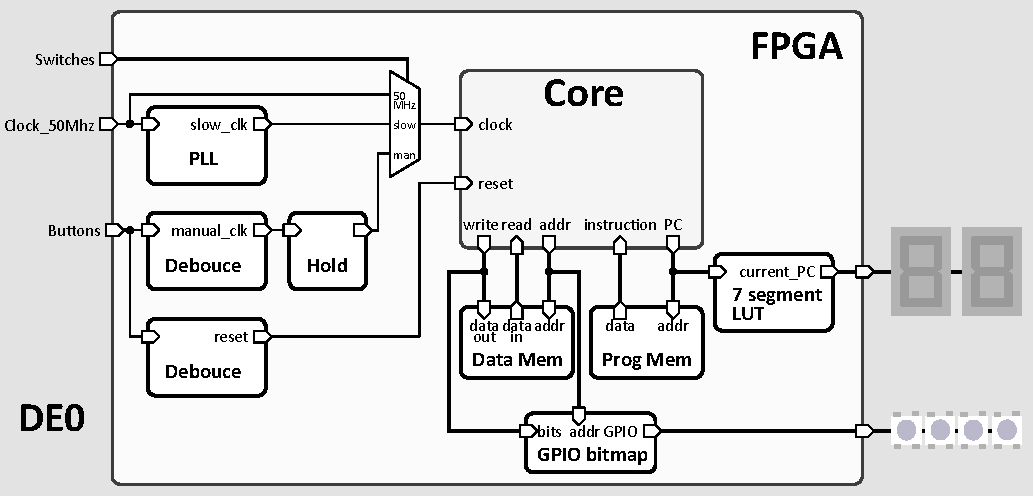
\includegraphics[width=0.9\linewidth]{pdf/arch_FPGA.pdf}
        \caption{Arquitectura de la FPGA. Esquema de blocs de la distribució i connexions entre les diferents elements.}
        \label{fig:FPGA_arch}
    \end{figure}
    
    El nucli per si sol no té manera de poder manifestar el seu funcionament més enllà de la modificació de dades de memòria. Per aquest motiu es necessari generar un mòdul que inclogui el nucli en qüestió i que es pugui comunicar amb la resta de l'entorn de desenvolupament, amb blocs de memòria ja existents proporcionats per l'entorn de síntesi, així com unitats de PLL per a acomodar el senyal de rellotge a freqüències baixes i poder seguir l'execució de manera fàcil. Altres elements que s'afegeixen són unitats que eliminen els rebots a l'hora de polsar botons per a poder aprofitar aquests senyals per a generar el rellotge o el senyal de reinici del nucli, o també l'adició d'un element que emula una unitat GPIO adreçada a una posició de memòria de manera que escrivint un valor en memòria el nucli pot encendre uns LEDs a la placa de desenvolupament. També s'ha afegit un sistema de monitorització per a identificar el PC actual.
    
    \subsection{Programació FPGA}
    Degut a que de moment el disseny del processador no permet carregar el programa de forma externa és necessari generar un fitxer d'iniciació de memòria per a poder deixar en el disseny verilog el programa ja càrregat i que aquest després sigui executat per el nucli. 
    Per a poder provar el funcionament de la FPGA a partir del nou model en Verilog preparat per a la placa de desenvolupament es procedeix a compilar el codi, sintetitzar-lo i generar la configuració especifica que s'haurà de càrregar a la FPGA per a obtenir el funcionament esperat. Aquest procés pot portar uns quants minuts i un cop complet genera un document que es pot utilitzar per a programar la FPGA. Un cop programada amb els elements físics de monitorització i de configuració del rellotge es pot arribar a determinar si realment el nucli està executant el programa de forma correcta.
    \subsection{Funcionament}
    
    Per a poder saber si el funcionament és correcte es pot reduir la velocitat del rellotge per anar seguint l'evolució del PC i verificar que els salts els fa correctament o directament generar un senyal de rellotge de manera manual.
    Per a verificar la càrrega i escriptura de dades a memòria es pot generar un programa que escriguí valors a memòria i aquest siguin utilitzats per a definir els valors de la paraula que està assignada al port GPIO per veure si els LEDs s'encenen de la forma esperada.
    *Foto FPGA amb leds encesos*

\section{Resum de resultats (desenvolupament i test)}
% Una secció on es presenti el mètode d’avaluació dels resultats, els resultats en si mateixos, i una discussió/reflexió sobre aquests resultats.

Per a provar el funcionament correcte del disseny s'han generat diferents tipus de proves.
Unes primeres a nivell de simulació en Verilog que consisteixen en generar paraules de programa, carregar-les a l'array intern de la memòria de programa, reiniciar el nucli i generar un senyal de rellotge durant certs cicles i analitzar l'estat d'algun registre intern o del PC i comparar-lo amb uns valors esperats. Aquesta aproximació permet generar les proves pròpies per a cada una de les instruccions del ISA i si en fer alguna modificació algun falla pots saber quin tipus d'operació falla i poder identificar de manera més ràpida l'error.

Un exemple d'aquest tipus de Testbench es prepar un petit programa que desi dos valors en dos registres interns, els sumi entre ells, el resultat es guardi en un tercer registre i al acabar l'execució verificar que a cert registre hi ha la suma dels dos primers valors. Per a poder generar les paraules del programa es poden utilitzar Tasks de Verilog que generin els 32 bits segons l'especificació per això poder parametritzar els elements de la instrucció i així poder-se utilitzar en altres tipus de test, com per exemple sumar un valor positiu i un de negatiu per verificar que les sumes amb signe funcionen. 

*Listing amb exemple de task i de test*

En canvi a l'hora de provar el funcionament en FPGA és necessari tenir certs mòduls provats com els d'escriptura de dades per a que el mòdul de GPIO pugui modificar l'estat dels LEDs segons el valor d'una posició de memòria. Però es pot generar un test fent un programa per exemple que executi un bucle (operacions de salt) incrementant un valor (registres + ALU) i el carregui i guardi a la posició de memòria on la unitat de GPIO està implementada i així poder veure físicament si el funcionament d'aquestes operacions funcionen en la implementació en FPGA. 

Normalment primer s'han provat els tests amb simulació abans de fer proves en FPGA.


\section{Metodologia}

Per a desenvolupar aquest treball final de grau primer s'ha fet una part important de recerca sobre la ISA de RISC-V, alguns exemples d'implementació tant teòrics com funcionals. Un cop feta aquesta recerca s'ha procedit a proposar diferents dissenys sobre el paper de l'arquitectura a alt nivell amb unitats definides molt a nivell de funcionament. Un cop acordat un disseny amb els tutors i la resta de l'equip ha començat un procés de programació en verilog del nucli primer a alt nivell determinant els blocs principals i certs senyals de control imposats per la ISA com el codi d'operació. Un cop aquesta versió inicial s'ha procedit a un procés iteratiu de modificació d'aquest dissenys afegint la funcionalitat per a les diferents instruccions del conjunt mentre paral·lelament s'anaven dissenyant els tests per a comprovar que les noves instruccions implementades funcionaven de manera correcta. Aquest procés ha sigut el més llarg degut a que a l'hora d'afegir noves instruccions succeïxen diferents problemes degut a decisions de disseny passades com l'amplada de diferents senyals de control o decidir en quina unitat implementar certa funcionalitat, amb reunions amb l'equip s'han anat consensuant aquestes dedicions de disseny. Un cop amb un disseny implementat per a tot el repertori s'ha començat a preparar la implementació en FPGA i l'adaptació a les memòries arbitràries. A la part final del projecte s'han fet els tests en FPGA que asseguren que el disseny funciona tant en simulació com en un entorn real.


\subsection{Flux de disseny}  % Correu1.2
Per a desenvolupar la metodologia anteriorment explicada s'ha intentat utilitzar software obert (excepte la implementació en FPGA degut a que la proporcionada només funciona amb software propietari) i aplicar tecnologies de gestió i automatització per a facilitar la detecció d'errors. 

Per a l'edició del codi Verilog s'ha utilitzat l'editor de text \textbf{Visual Studio Code} (VSC) degut a que és de codi obert i permet afegir extencions que són de gran ajuda a l'hora de poder desenvolupar el projecte, en concret s'ha utilitzat una extensió anomenada ``\textbf{Verilog HDL/SystemVerilog}'' \ref{} que permet executar una aplicació de \textbf{linting} \ref{} (anàlisi d'errors en el codi) en temps real que ajuda molt a no haver de guardar el codi i executar-lo externament i analitzar la sortida del compilador per a detectar errors. Com a compilador de verilog s'ha utilitzat \textbf{Icarus Verilog} degut a que es una implementació opensource i permet executar testbench des de la línia de comandes. Per a executar els tests s'ha fet un petit script en \textbf{bash} per a llançar-lo de com a tasca de compilació des de VSC. 

A l'hora de manejar el codi del propi nucli s'ha utilitzat \textbf{git} per a poder tenir un històric del desenvolupament i informació de les modificacions que s'anaven fent al projecte. Per a assegurar-se que el disseny passa els tests i automatitzar-ne el proces s'ha utilitzat \textbf{docker}, \textbf{Icarus Verilog} i \textbf{Travis} per a poder generar un contenidor capaç d'executar els tests (docker + icarus verilog) i l'automatització amb Travis ja que proporciona el còmput i integració amb github que permet que amb cada modificació s'aixequi la imatge de docker abans creada i verifiqui el funcionament informant en cada commit. 

Aquesta primera part basat en el diseny i test a nivell de simulació. A l'hora de fer sintesi el proces es basa incialment de la mateixa manera, important els documents Verilog del nucli però en l'aplicació \textbf{Quartus II} d'Altera. En aquesta aplicació s'ha desenvolupat l'entorn per a que el nucli pugui interaccionar amb la placa de desenvolupament \textbf{DE0} de TerAsic guardant els canvis en el mateix repositori de github però sense executar tests ja que l'aplicació Quartus ii és propietària i els tests s'han de fer en físic amb la FPGA.

Per a generar els codis de programa per als tests de la FPGA s'ha utilitzat el \textbf{riscv-gnu-toolchain} dins una imatge de Docker (per a no haver de tornar a compilar tot l'entorn cada cop) per a partir d'un codi en C poder compilar-lo amb \textbf{GCC} al repertori RV32I i poder posar el codi resultant com a inicialització de la memòria de programa de la FPGA.

\section{Conclusions i treball de futur}  % Correu1.3

Mirant els objectius principals d'aquest projecte es pot dir que s'han assolit, degut a que s'ha entregat un disseny de nucli RISC-V que implementa la extensió RV32I, el disseny està provat a nivell de simulació i a nivell físic amb la implementació de la FPGA. També s'han utilitzat eines que s'han après al llarg de la carrera per a facilitar el manteniment de codi i/o la facilitat de poder utilitzar codi en contenidors i sistemes d'integració contínua per a rebre avisos si no es passen correctament els tests.

A nivell de coneixements s'ha ampliat molt el coneixement de RISC-V i el desenvolupament de processadors a nivell de RTL. Sobretot el principi de ``learning by doin'' fa que s'entenguin els conceptes en profunditat ja que pots veure com implementar un concepte a mitges pot provocar un funcionament no esperat, com es el cas amb les memòries.

Com a treball futur es pot revisar i optimitzar el disseny del propi processador, sobretot simplificar la unitat de CSR ja que s'ha implementat de manera funcional i no es massa òptim i degut a que es una unitat que pot ser fàcilment extensible amb comptadors extres és millor utilitzar codi més simple.

També es pot millorar les prestacions del propi processador afegint pipeline per a poder executar diferents instruccions a l'hora i poder augmentar el rendiment.

Degut a que aquest nucli es vol utilitzar per a un projecte que permeti veure l'estat del processador en tot moment i poder modificar-ne l'estat del mateix dissenyar un entorn de debug al voltant del nucli és un pas evident per a aconseguir aquesta funcionalitat.
    
    



\section*{Agraïments}

... ..  .... .. .... ... ..... ... ..... ... ... ..... .... .
.... ..  .... .. .... ... ..... ... ..... ... ... ..... .... .
.... ..  .... .. .... ... ..... ... ..... ... ... ..... .... .
.... ..  .... .. .... ... ..... ... ..... ... ... ..... .... .
.... ..  .... .. .... ... ..... ... ..... ... ... ..... .... .


\bibliographystyle{IEEEtran}
\bibliography{references.bib}

%\begin{thebibliography}{11}
%\bibitem{latex}
%http://en.wikibooks.org/wiki/LaTeX

%\bibitem{2}
%Referència 2

%\bibitem{3}
%Etc.


%\end{thebibliography}

\appendix

\section*{Apèndix}

\setcounter{section}{1}

\subsection{Secció d'Apèndix}
% Utilitzeu el begin table només en cas de vole taules flotants. Si les voleu al lloc, tabular directament.
\begin{table}[h]
\caption{Taula d'exemple}
\label{tab:senzilla}
\begin{center}
\begin{tabular}{|c|c|}
\hline
One & Two\\
\hline
Three & Four\\
\hline
\end{tabular}
\end{center}
\end{table}

... ..  .... .. .... ... ..... ... ..... ... ... ..... .... .
.... ..  .... .. .... ... ..... ... ..... ... ... ..... .... .
.... ..  .... .. .... ... ..... ... ..... ... ... ..... .... .
.... ..  .... .. .... ... ..... ... ..... ... ... ..... .... .
.... ..  .... .. .... ... ..... ... ..... ... ... ..... .... .

\subsection{Secció d'Apèndix}


... ..  .... .. .... ... ..... ... ..... ... ... ..... .... .
.... ..  .... .. .... ... ..... ... ..... ... ... ..... .... .
.... ..  .... .. .... ... ..... ... ..... ... ... ..... .... .
.... ..  .... .. .... ... ..... ... ..... ... ... ..... .... .
.... ..  .... .. .... ... ..... ... ..... ... ... ..... .... .


\end{document}

